\chapter{Introducción} % (fold)
\label{cha:introduccion}

\section{Motivacion} % (fold)
\label{sec:motivacion}

\begin{itemize}
	\item Económico:
	    \begin{itemize}
	        \item Materiales a nuestro alcance.
	        \item Posibilidad de realizar un producto viable.
	    \end{itemize}
	\item Académico:
	    \begin{itemize}
	        \item Oportunidad de mejorar y facilitar las mediciones de sensores analógicos y recolectar datos de señales digitales para los alumnos que realicen proyectos en el LAC (Laboratorio de Arquitectura de Computadoras)
	    \end{itemize}
	\item Investigación:
	    \begin{itemize}
	        \item Investigar como acelerar los procesos de desarrollo de software y hardware.
	        \item Poner en uso una metodología ágil en el software.
	        \item Poner en uso una metodología ágil en el hardware.
	    \end{itemize}
	\item Extensión:
	    \begin{itemize}
	        \item Laboratorios de Universidades de la RUNIC.
	        \item Empresas del medio.
	    \end{itemize}
	\item Tecnológico:
	    \begin{itemize}
	        \item Utilizar tecnología madura.
	        \item Utilizar tecnología bien documentada y dejar bien documentado nuestro sistema.
	        \item Utilizar tecnología muy difundida.
	    \end{itemize}
\end{itemize}

% section motivacion (end)

\section{Objetivos} % (fold)
\label{sec:objetivos}

\subsection{Objetivos Principales} % (fold)
\label{sec: objetivos_funcionales}

\begin{itemize}
    \item Diseñar y construir una placa para el sensado de señales analógicas y digitales.
    \item La placa debe leer entre 8 y 16 señales analógicas.
    \item La placa debe contar eventos digitales con 2 o 3 contadores distintos.
    \item La placa debe transmitir los datos digitales a través de un protocolo serial, a alguna otra placa de desarrollo o procesador.
\end{itemize}

% section objetivos_principales (end)

\subsection{Objetivos Secundarios a Alcanzar en el Tiempo Estimado} % (fold)
\label{sec: objetivos_secundarios}

\begin{itemize}
    \item El sistema debe poder ser configurado con parámetros de ganancia (amplificación de señal analógica de entrada), decidir que pin se utilizara como entrada y respecto a que (masa o si mismo), se realizara la medición.
    \item Lograr que el sistema tenga el menor consumo posible.
    \item Lograr que el sistema tenga la mejor inmunidad al ruido posible.
    \item El sistema debe ser lo mas pequeño posible.
    \item Se debe poder aplicar al sistema un sensor de campo electrostático, provisto por el FAMAF.
    \item El sensor de campo electrostático debe tener una placa por separado para el manejo de la potencia.
    \item Se debe controlar la velocidad del motor del sensor desde el software incluido en el microcontrolador.
    \item Se debe desarrollar un servidor web en alguna placa de desarrollo para poder controlar todas las acciones del sensor remotamente.
    \item El servidor web debe poder guardar datos de las lecturas que se realizan del sensor en una base de datos (preferentemente MySQL).
    \item Escribir la documentación sobre las instrucciones de uso para manejar el software embebido en la placa.
    \item Realizar una prueba de campo.
\end{itemize}

% section objetivos_secundarios (end)

\subsection{Objetivos para un Futuro Prototipo} % (fold)
\label{sec: objetivos_futuros}

\begin{itemize}
    \item Poder mejor la placa utilizando un microcontrolador mas potente.
    \item Mejorar la reacción del sistema ante fallos de potencia.
    \item Mejorar el prototipo del sensor de campo electrostático para reducir el consumo y el ruido.
    \item Mejorar el servidor web para sensores en general.
    \item Mejorar el servidor web para incluir gráficos.
\end{itemize}

% section objetivos_futuros (end)

\section{Herramientas de modelado} % (fold)
\label{sec:herramientas_de_modelado}

Para facilitar la documentación, decidimos utilizar SysUML para documentar nuestro sistema. Para esto, utilizamos la herramienta Enterprise Architect, que nos permite partir de un modelo base y reutilizar los componentes en todos los diagramas, generando vínculos que facilitan el entendimiento general del sistema.

% section herramientas_de_modelado (end)

\section{Requerimientos} % (fold)
\label{sec:requerimientos}

\subsection{Requerimientos funcionales} % (fold)
\label{sub:requerimientos_funcionales}

\begin{itemize}
	\item Se debería poder recibir datos de sensores analógicos en modo singular o equilibrado
	\item Se debería poder contar eventos de señales digitales cuadradas
	\item Se debería poder configurar una ganancia especifica y un tiempo entre mediciones especifico para cada entrada
	\item Los parámetros que corresponden a la ganancia, el modo de conversión, el tiempo entre conversiones, y la cantidad de canales habilitados para la conversión y el conteo de eventos, deberían ser configurables a través de una interfaz de linea de comando
	\item Se debería usar un protocolo serial para la interfaz de linea de comando entre el sistema y el usuario
	\item El usuario debería poder configurar el sistema conectándolo a un ordenador u otro sistema que soporte comunicación serial.
	\item Se debería poder enviar datos de mediciones y posibles meta-datos a través de un canal de comunicación mediante un protocolo serial.
\end{itemize}

% subsection requerimientos_funcionales (end)

\subsection{Requerimientos no funcionales} % (fold)
\label{sub:requerimientos_no_funcionales}

\begin{itemize}
	\item Debería consumir lo menos posible
\end{itemize}

% subsection requerimientos_no_funcionales (end)

% section requerimientos (end)

\section{Características generales} % (fold)
\label{sec:caracteristicas_generales}

En una primera aproximación del sistema a construir, se puede establecer que se trata de un sistema capaz de recibir señales de distintos sensores digitales y analógicos. En caso que sean analógicos, convertir las señales a digital usando un conversor A-D de alta ganancia, que permita tanto entradas singulares como equilibradas. Luego de ser convertidas, estas señales deben ser enviadas mediante un protocolo serial a otro sistema que realice las acciones que deba realizar en función de los datos enviados.

Se puede establecer que en nuestro contexto interactúan 3 actores: Un usuario, uno o mas sensores, y un controlador que por el momento no hacemos mención de sus características, por lo que lo llamamos simplemente ``controlador''.

\begin{figure}[h]
  \centering
  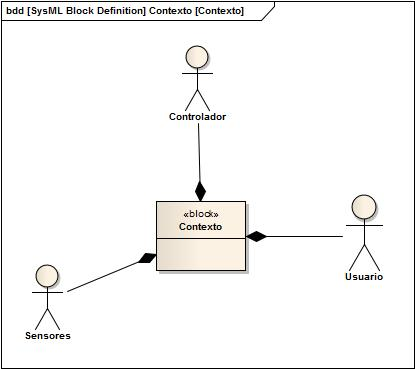
\includegraphics[width=0.80\textwidth, height = 9cm]{contexto1}
  \caption{Contexto del sistema}\label{fig:contexto1}
\end{figure}

% section caracteristicas_generales (end)

\section{Metodo de desarrollo} % (fold)
\label{sec:metodo_de_desarrollo}

El método de desarrollo utilizado es el desarrollo iterativo con entrega incremental. Este modelo se ilustra en la figura \ref{fig:MetodoDeDesarrollo}. En esta metodología de desarrollo el trabajo se divide en iteraciones en las cuales el producto va evolucionando. 
Un aspecto fundamental para guiar el desarrollo incremental es la priorización de los requerimientos/objetivos en función del valor que aportan al cliente. De esta manera se van añadiendo nuevos requerimientos o mejorando los que ya se completaron. Al finalizar cada iteración se obtiene un prototipo funcional.

\begin{figure}[h]
  \centering
  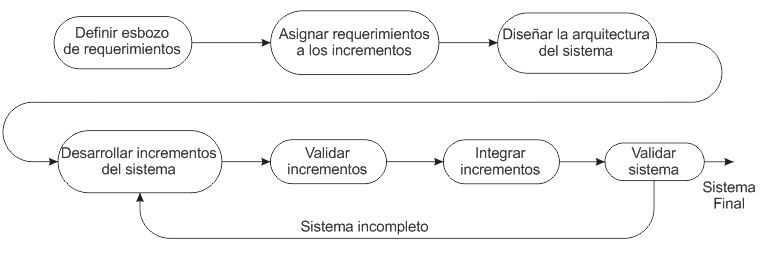
\includegraphics[width=0.80\textwidth, height = 4cm]{MetodoDeDesarrollo}
  \caption{Desarrollo incremental}\label{fig:MetodoDeDesarrollo}
\end{figure}

% section metodo_de_desarrollo (end)

\section{Casos de uso} % (fold)
\label{sec:casos_de_uso}

Dado el contexto, el sistema se puede describir de una manera general mediante un diagrama de caso de uso. El diagrama puede verse en la figura \ref{fig:casouso1}. En esta figura, se pueden ver los requerimientos plasmados en los casos de uso.

\begin{figure}[h]
  \centering
  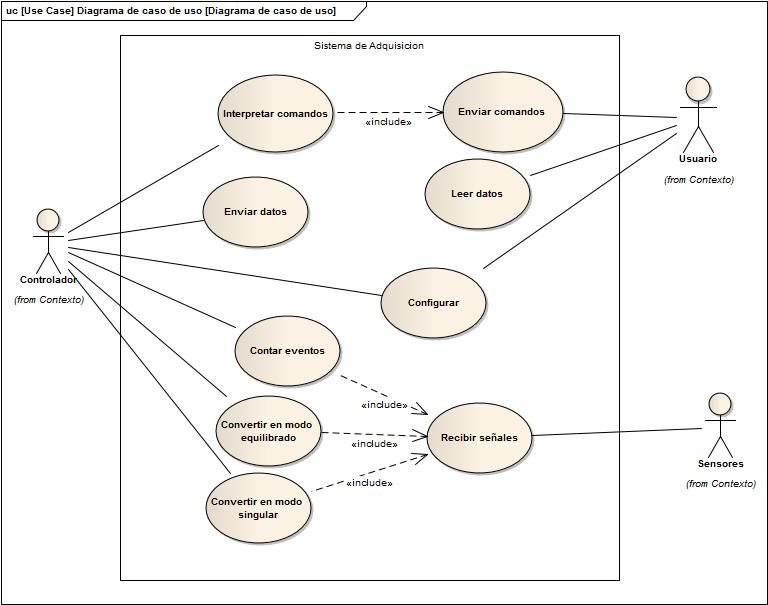
\includegraphics[width=0.80\textwidth, height = 11cm]{casouso1}
  \caption{Diagrama de caso de uso del sistema de adquisición}\label{fig:casouso1}
\end{figure}

El caso de uso ``configurar'' esta generalizado. Las acciones que incluye este caso son:
\begin{itemize}
	\item Configurar la interfaz serial
	\item Configurar canal en modo singular
	\item Configurar canal en modo equilibrado
	\item Configurar contador de eventos
	\item Configurar ganancia del del conversor
	\item Configurar intervalo de medicion para conversion analogica
\end{itemize}

% section casos_de_uso (end)

% chapter introduccion (end)